\section{Etat de l'art}

%%%%%%%%%%%%%%%%%%%%%%%%%%%
%  Historique SSL/TLS     %
%%%%%%%%%%%%%%%%%%%%%%%%%%%

\begin{frame}{Historique des attaques sur SSL/TLS}
    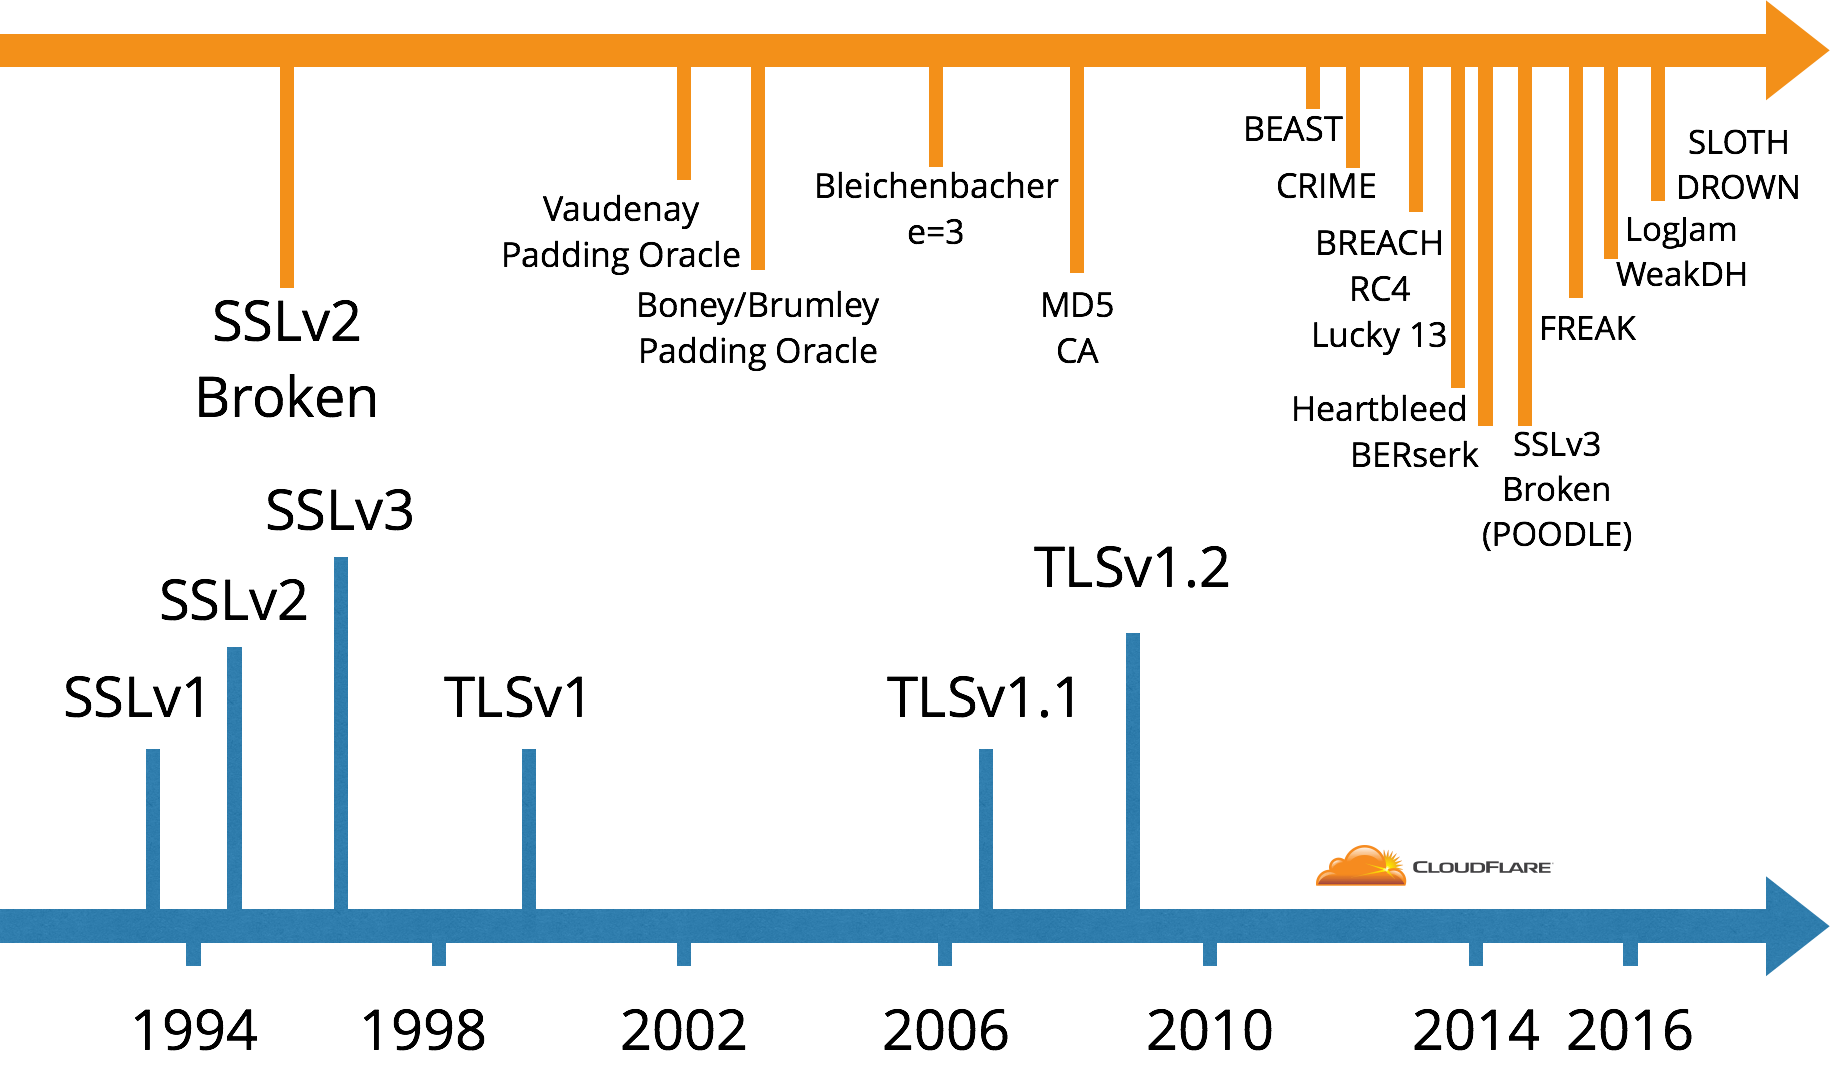
\includegraphics[width=\linewidth]{../medias/history-tls-attacks.png}
\end{frame}

%%%%%%%%%%%%%%%%%%%%%%%%%%%
%  Attaques HTTPS         %
%%%%%%%%%%%%%%%%%%%%%%%%%%%

\begin{frame}{Attaques sur HTTPS}

  {\Large \centerline{Plusieurs angles d'attaques :}}

  \begin{columns}
    \begin{column}{0.5\textwidth}
      \begin{exampleblock}{Failles d'implémentation}
        \begin{itemize}
        \item Bibliothèques (openssl)
        \item Navigateurs (Internet Explorer)
        \end{itemize}
      \end{exampleblock}

      \begin{exampleblock}{Cryptographie}
        \begin{itemize}
        \item Mode de chiffrement (CBC)
        \item Algorithmes (RC4)
        \end{itemize}
      \end{exampleblock}

      \begin{exampleblock}{Protocole}
        \begin{itemize}
        \item{Downgrade attack (POODLE)}
        \end{itemize}
      \end{exampleblock}
    \end{column}

    \begin{column}{0.5\textwidth}
      \begin{figure}
        
\includegraphics[width=0.32\linewidth]{../medias/heartbleed.png}
      \end{figure}
      \begin{figure}
        
\includegraphics[width=0.32\linewidth]{../medias/sweet32.png}
      \end{figure}
      \begin{figure}
        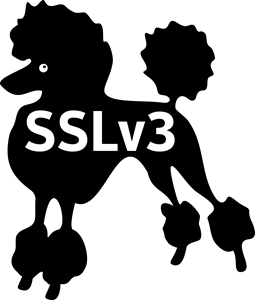
\includegraphics[width=0.32\linewidth]{../medias/poodle.png}
      \end{figure}
    \end{column}
  \end{columns}

\end{frame}
